\chapter{Un fruit du « pré-réformisme » : le wahhabisme}
\mn{ \emph{(31/01/2022)}}

%---------------------------------------------------------
\section{Le wahhabisme}
\paragraph{Pourquoi en parler} C'est un courant qui a presque trois siècles, avec une évolution dans le monde du musulman qui a évolué. Il faut penser l'Islam contemporain dans son contexte.

 
  \subsection{Muhammad Ibn al Wahhab
  (1702-1792)} 
  \label{Theol:AlWahhab}
  
\paragraph{Origine} Son père est \emph{qadi}\sn{juge} et enseignant. Dans le Hadz. Fait un pélerinage à la Mecque. Renouveau

\paragraph{Formation et premières prédications} Proclame le \emph{Tawhid} l'unicité et lutte contre toutes les pratiques "déviantes". Il se heurte aux autorités locales et retourne donc à la Mecque. Il se forme là avec des maîtres d'Arabie et Indien. Puis se rend à Basra, à un autre maître. C'est là qu'il rencontre les si'ites. Il se heurte de nouveau aux autorités locales. Il rentre en Arabie mais \textit{son père y est hostile}. Ce n'est pas un grand savant mais un lettré. 
 
\paragraph{L'alliance avec Ibn Se`ud} Alliance matrimoniale avec un chef de tribu de la Mecque. Il se rend indésirable et il est obligé de partir et il arrive dans le village de Dariya et il y rencontre un autre chef de village, Mohammed Ibn Se'ud, alliance elle aussi politicolo-religieuse et matrimoniale en 1744. Ibn Se'ud accepte la doctrine et al Wahhab légitime l'acquisition de terre par Ibn Se'ud. 

Wahhab enseigne beaucoup  : il écrit beaucoup à des savants (\emph{Oulema}) à l'intérieur et l'extérieur du royaume de Ibn Se'ud. \textit{selon un modèle prophétique}, Mohammad ayant écrit au Basileos,... 

\paragraph{Un développement politique} Conquiert toute l'Arabie Saoudite. En 1818, c'est la fin du premier état wahhabite car l'empire ottoman intervient et execute le fils de Ibn Se'ud.
    
 Il s'appuie sur deux auteurs : 
\begin{itemize}
    \item Ibn Taymiyya (1263-1328), \label{Theol:Taymiyya2} \sn{cf p. \pageref{ibn-taymiyya}}, un vrai penseur
    \item Ibn Qayyim (1292-1350) un de ces disciples
\end{itemize}
 
Ibn Wahhab insiste sur le retour à la source mais en fait il lit le Coran à travers ces deux auteurs.

\paragraph{Une doctrine condamnée} Son père et son frère s'opposent à lui. Une fatwa contre lui du fait de sa critique sur les différentes écoles juridiques et le fait qu'il exclut de la communauté musulmanes ceux qui ne pensent pas comme lui. 

  \subsection{La doctrine wahhabite} 



  \paragraph{Nécessité du retour aux sources} Accentuation des sources, bien sûr le Coran. 
  \begin{itemize}
      \item  \item  Wahhab s'éloigne d'une lecture du Coran ligne à ligne mais propose une analyse \textit{thématique}.
  \item Il rejette aussi le besoin d'une \textit{médiation} humaine pour comprendre le Coran. Il s'oppose aux \emph{Ashraf}, les descendants du prophète \sn{Les Ashrafs ont un statut particulier dans l'Islam} ainsi qu'aux \emph{Imams} dans le si'isme, ainsi que les \emph{sheykhs} soufis.
  \begin{Prop}
  Il n'y a pas besoin de sciences particulières pour accéder au sens du Coran, d'après Wahhab. 
  \end{Prop}
  \item il suis les \emph{Hadiths}, la seule exégèse possible, la \textit{sunna} et rejette les grands commentaires classiques du Coran.  Cela va jusqu'à critiquer la tradition des 4 premiers Califes \textit{bien guidés}. Abu Bakr avait détourné la \textit{zakat} pour ses propres dépenses.
  \item Il reprend la distinction d'Ijtihad, qu'il limite aux versets aux versets obscures, contre le taqlid. Il s'oppose à deux principes de l'Ijtihad : qiyas (recours par analogie : alcool et drogue), \textit{ijama} (consensus des savants : on considère que cela fait autorité \sn{Infaillabilité de la communauté dans les Hadiths}), et le \textit{ra'y}, l'opinion personnelle du juriste. 
  
  \end{itemize}
 
 \begin{Prop}
 Il conteste les principes sous-jacents aux savants qui l'ont précédés. Il y a une tension entre son ambition de revenir au Coran mais en parallèle en se mettant en filiation avec Ibn Taymiyya
 \end{Prop}
 
 
  \paragraph{Une notion centrale : le \emph{tawhid} (unicité divine)}
  
  \mn{{Extraits du \emph{Kitab at-tawid} (Livre de
l'unicité divine) de Muhammad Ibn Wahhab} . {Chapitre 1} : \emph{Tawhid}
Traduction et édition établies en Arabie Saoudite. Allah est traduit par Allah et non Dieu, alors qu'en Arabe, Dieu est traduit par Allah y compris pour les chrétiens arabes. }

\begin{quote}
\emph{Allah-ta`ala} a dit : « Je n'ai créé les djinns et les hommes que
pour qu'ils M'adorent (1 :56)\ldots Et très certainement nous avons
suscité dans chaque communauté un message pour leur dire d'adorer Dieu
et d'écarter le Rebelle (16 :36)\ldots Et voilà que ton Seigneur a
décrété que tu dois n'adorer que Lui et faire preuve de bonté envers tes
parents (17 :23)\ldots Adorez Dieu et ne lui donnez quelque associé que
ce soit (4 :36)\ldots Venez, je vais vous réciter ce que votre Seigneur
vous a interdit ; - ceci : Ne lui associez quoi que ce soit\ldots(6
:151-153) ». Ibn Mas`ud a dit : « Quiconque se propose de vérifier le
testament du Prophète Muhammad (SWA) -- un testament sur lequel le
Prophète a apposé son sceau, qu'il lise ces mots d'Allah : « Venez, je
vais vous réciter ce que votre Seigneur vous a interdit ; - ceci : Ne
lui associez quoi que ce soit\ldots Voilà ce qu'il enjoint » (6 :
151-153)


Mu`adh Ibn Jabal raconta : « Je montai derrière le Prophète (SAW) quand
il me dit : « Ô Mu`adh ! Sais-tu ce que les créatures d'Allah Lui
doivent et ce qui leur est dû ? » Je répondis : « Allah et son Prophète
savent mieux ». Il continua : « Ce que les créatures d'Allah Lui
doivent, c'est de ne jamais associer qui que ce soit avec Lui. Ce qui
leur est dû, c'est qu'il ne punira aucune personne qui ne Lui associe
pas un autre ». Je dis :

« Ô Prophète d'Allah, est-ce que je peux annoncer la bonne nouvelle aux
gens ? » Il répliqua : «Non ! Ne leur dis rien de peur qu'ils comptent
sur la promesse et manquent à leurs devoirs envers Lui». Ce hadith est
mentionné dans deux \emph{Sahihs}.


D'autres points :


\begin{enumerate}

\item
  \begin{quote}
  La sagesse dans la création du djinn et de l'humanité.
  \end{quote}
\item
  \begin{quote}
  Le service à Allah consiste en le \emph{tawhid}. Car, à l'opposé du
  \emph{tawhid} se trouve l'aliénation d'Allah. (\ldots)
  \end{quote}
\item
  \begin{quote}
  La sagesse d'envoyer des prophètes. (\ldots)
  \end{quote}
\end{enumerate}
  \end{quote}
  
On trouve une accumulation de versets coraniques sur le thème, puis des hadiths du prophète. Le grand péché par excellence, c'est le \emph{shirk}, l'associationisme des Dieux à Dieu. Or Wahhab va plus loin. 

\begin{quote}


\emph{Allah-ta`ala} dit : « Ceux qui ont cru et n'ont point revêtu de
prévarication leur foi\ldots{} » (6 : 82).

(\ldots) Abu Sa`id al Khudriyy rapporta que le Prophète d'Allah (SWA) a
dit : « Quand Musa {[}Moïse{]} demanda à Allah de lui enseigner une
prière qu'il puisse réciter à chaque fois qu'il pensait à Lui ou qu'il
L'évoquait, Allah répondit : « Dis, ô Musa, qu'il n'y a d'autre Dieu
qu'Allah. Musa dit : « Ô Seigneur, tous tes serviteurs prononcent ces
mots ». Allah dit : « Ô Musa, si les sept cieux et tout ce qu'ils
renferment, et les sept terres aussi, si tout cela était pesé contre
cette phrase : « Il n'y a d'autre Dieu qu'Allah », cette dernière
pèserait plus lourd ». Ibn Hibban rapporta cela également et al-Hakim
compléta sa version. Al-Tirmidhi enregistra, avec peu de rédaction, le
récit de Anas à l'effet qu'il entendit le Prophète d'Allah (SWA) dire :
« Allah dit : « Ô Homme ! Si tu venais à Moi avec tous les sacs du monde
remplis de tes péchés, mais avec le témoignage que tu n'associes rien à
Moi, Je viendrais à toi avec tous mes sacs remplis de miséricorde et de
pardon ! ».

    
\end{quote}

\begin{Synthesis}
Si on respecte le \emph{Tawhid}, cela suffit à pardonner les péchés, mais important de respecter les principes de l'Islam (c'est pour cela que c'est caché)
\end{Synthesis}

\paragraph{Distinction au sein du Tawhid } 
\begin{Def}[Le grand Shirk ]
Il distingue le \emph{tawhid rububiyya} (l'unicité de souverainté du monde) avec le \emph{tawhid uluhiyya} (de divinité) : ne reconnaitre aucun intermédiaire entre Dieu et les hommes. Il ne peut y avoir de dévotion que pour Dieu seul : les saints, les soufis, les Imams.
\end{Def} 
Al Wahhab introduit une critique fondamentale contre le soufisme. 

\paragraph{Le petit Shirk} 
\mn{{Chapitre 4} : La crainte du \emph{shirk}}
\begin{quote}
Allah -- qu'Il soit loué et glorifié -- dit : « Non, Dieu ne pardonne
pas qu'on Lui donne quelque associé. En deçà, Il pardonne à qui il veut
» (4 : 48, 116)

(\ldots) Dans le hadith, nous lisons : « Ce que je crains le plus pour
vous, c'est le moindre \emph{shirk}. Quand on lui demanda ce que
c'était, le Prophète répondit : « l'hypocrisie ». Dans le Sahih
d'al-Bukhari, nous lisons que Ibn Mas`ud reporta : « Le Prophète d'Allah
(SWA) a dit : « Celui qui rencontre Allah le jour du Jugement sans Lui
avoir associé qui que ce soit ira au Paradis, et celui qui le rencontre
ayant fait le contraire sera consigné en Enfer ».
\end{quote}
\begin{Def}[le Petit Shirk]
Toute attitude de l'homme qui ne sert pas Dieu. il relève aussi de l'attitude morale.
\end{Def}

\begin{Ex}[L'appel à témoigner qu'il n'y a d'autre
Dieu qu'Allah]

\mn{{Chapitre 5} : }
\begin{quote}
\emph{Allah-ta`ala} a dit : « Dis (ô Muhammad) : `\,`Voici mon sentier,
j'appelle à Dieu'\,' » (12 :108)

Ibn `Abbas (RA) rapporta : « Quand le Prophète d'Allah (SAW) envoya
Mu'adh à al-Yaman, il lui recommanda : `\,`Quand tu rencontres des gens
du Livre, que ta première action soit de leur demander de témoigner
qu'il n'y a d'autre Dieu qu'Allah'\,' ». Selon un autre récit, «
\ldots{} de leur demander de réaliser l'unicité d'Allah. S'ils
t'obéissent, informe-les qu'Allah leur a imposé la \emph{salat} cinq
fois par jour. S'ils t'obéissent en cela, alors informe-les qu'Allah
leur a imposé le devoir de charité qui doit être perçue des riches pour
être distribué aux pauvres. S'ils t'obéissent en cela, ne touche pas à
leurs autres biens et occupe-toi de la plainte de l'opprimé, car il n'y a aucun obstacle dans son accès à Allah ».
(Rapporté dans les \emph{Sahihs} d'al-Bukhari et de Muslim). (\ldots)
\end{quote}
\end{Ex}



\paragraph{Les Intercessions} L'intercession est limitée à Mohammed, et uniquement aux musulmans suivants Wahhab. On ne peut pas prier le Prophète. Peut être intervient-t-il au jugement dernier.


\mn{{Chapitre 17} : L'intercession}
\begin{quote}
Allah -- qu'il soit loué et glorifié -- a dit : « Et par ceci (le
Qur'an), avertis ceux qui, n'ayant pour eux hors de Dieu, ni ami ni
intercesseur, craignent d'être rassemblés vers le Seigneur\ldots{} » (6
: 51). Dis : « A Dieu l'intercession tout entière\ldots{} » (39 : 44).
Qui peut intercéder auprès de Lui que par sa permission ?... (2 : 255).
Et combien d'anges dans les cieux ? Leur intercession ne met au large en
rien, sauf après que Dieu l'a permis, en faveur de qui il veut et qu'il
agrée » (53 : 26). (\ldots)

(\ldots) En tant que catégorie générale du Jour du Jugement en laquelle
les mécréants croient, l'intercession est rejetée par le Qur'an. Le
Prophète (SAW) nous informa qu'en ce jour « il sera amené devant Allah.
Il se prosternera lui-même et louera Allah, plutôt que de demander à
intercéder. Alors on lui dira : « Lève-toi ! Parle maintenant et tu
seras entendu ! Demande et il te sera donné ! Intercède et il te sera
accordé ! » (\ldots) L'intercession est donc là pour les croyants
sincères et candides. Elle n'est accordée que par la permission d'Allah
et n'appartient pas aux associationistes. (\ldots)
\end{quote}


\paragraph{Tombe du juste}
Condamnation de celui qui invoque Dieu
auprès de la tombe du juste et, a fortiori, de celui qui invoque ce
dernier.
\begin{Ex}[Un exemple de Grand Shirk]
\mn{{Chapitre 20} : Condamnation de celui qui invoque Dieu
auprès de la tombe du juste et, a fortiori, de celui qui invoque ce
dernier.}
\begin{quote}
Dans le \emph{Sahih}, A'ishah (RAA) rapporta : « Umm Salmah raconta au
Prophète d'Allah (SAW) qu'elle avait vue une église remplie d'images et
de statues en Abyssinie. Le Prophète dit : « Ceux-là sont les pires de
tous les hommes : lorsqu'un membre juste et vertueux de leur groupe
meurt, ils bâtissent une église sur sa tombe et y installent toutes
sortes d'images pour lui. Ils sont coupables de deux méfaits : celui
d'invoquer quelqu'un auprès d'une tombe et celui d'installer des images
». (\ldots)

Ainsi le Prophète interdit cette pratique et condamna celui qui la
suivait. Faire le \emph{salat} sur une tombe est également interdit,
même si aucune mosquée n'a été construite sur l'emplacement. Telle est
la signification de la déclaration suivante : « On craignait qu'elle ne
soit prise pour une mosquée ». Les Compagnons n'étaient pas supposés
construire une mosquée autour de la tombe du Prophète. Tout endroit
destiné au \emph{salat} ou tout endroit où le \emph{salat} est accompli,
est une mosquée. Tel l'a déclaré le Prophète (SAW) : « Toute la terre
est pour moi une mosquée, un endroit pur (pour accomplir le
\emph{salat}) ».
\end{quote}

\end{Ex}


  \paragraph{La question du \emph{jihad}} La question de la violence chez Wahhab. Il faut repartir de la position kharijite. Un calife doit respecter la religion de façon exemplaire. s'il ne le fait pas, il est \emph{Takfir}, mécréant. Or la vision sunnite a jugé que c'est Dieu uniquement qui jugera si un musulman est un non-musulman. Ibn Taymmayyia s'élève contre les souverains Mongols : : les souverains mongols sont certes musulmans puisqu'ils ont adopté la foi musulmane mais en surface.  Wahhab va reprendre ce concept et ceux qui n'adhèrent par au \emph{shirk} sont apostats. Un germe de violence.
  
  \begin{Synthesis}
  On voit donc l'extension du concept de Ibn Taymmayyia sur le Takfir à tout le shirk, et donc en pratique en non respect du wahhabisme.
  \end{Synthesis}
 
 Mais il n'y a pas de volonté de jihad dans le wahhabisme. On peut même faire des traités avec des non-musulmans.
 
  \section{Le devenir du wahhabisme} 
 
  
 

% ------------------------------ 
\subsection{Les trois Etats Saoudiens} 

 
  {\paragraph{1744 -1818}: une première expansion}
 
 
\emph{1744} alliance Ibn Se`ud /Ibn al-Wahhab
 
\emph{1786} conquête du Najd (`Abd-al-`Aziz)
 
\emph{1792} mort d'Ibn al-Wahhab
 
\emph{1806} conquête de La Mecque
 
\emph{1818} défaite devant les Ottomans
 

 
  {\paragraph{1821-1883}: petit Etat centré sur Riyad (Najd)}
 
  {\paragraph{1901- 2011} : le Royaume d'Arabie Saoudite} Un descendant de Wahhab qui repasse alliance avec la famille de Se'ud et conquiert l'Arabie. 
 
 
\emph{1924} conquête de La Mecque. Abdelaziz Ibn Se`ud prend le titre de
roi et \textit{protecteur des lieux saints}. On détruit les confrérie, on contrôle le pélerinage, on supprime les autres écoles de droit.

\mn{REVOIR}

\emph{1939} début de la production pétrolière \emph{1962} création de la
Ligue islamique \emph{1990} début de la guerre du Golfe.
 

 
\subsection{L'Arabie Saoudite et l'économie
pétrolière} 
 
\paragraph{ {Début de la
production}} 

\begin{quote}
1935: premier forage

1939: premier baril de pétrole

⇒ Cartel américain: l'ARAMCO
\end{quote}

 
\paragraph{{Nationalisation de la
production}}


1973: l'Etat s'approprie 25 \% des droits de l'ARAMCO (1974 : 60\%, 1980 : 100\%)


⇒ Saoudi ARAMCO: 95 \% de la production du pays.

 
\paragraph{Evolution du cours du
pétrole} 

\begin{quote}
1973: premier choc pétrolier (guerre de Kippour) =\textgreater{} de 4 à
15 \$/B

1981-1983: deuxième choc pétrolier (Révolution iranienne + guerre
Iran-Irak) =\textgreater{} 36 \$/B 2006-2008: troisième choc pétrolier
(guerre en Irak) =\textgreater142 \$/baril
\end{quote}

\paragraph{{Rente}}: 1973-2002 =\textgreater{} 200 000 milliards
de dollars au total
 
    Une étude de cas : le wahhabisme en Afrique de l'Ouest
    
\subsection{Le wahhabisme et l'Etat saoudien}

Le wahhabisme accepte une certaine ouverture en Arabie en contrepartie de financement extérieur. On est dans des \textit{concessions} des oulemas. 

\paragraph{La ligue islamique 1962} on étudie gratuitement à la Mecque et à Médine pour propager le wahhabisme.

 
\subsection{Une étude de cas : le wahhabisme en Afrique de l’Ouest}

\paragraph{Des étudiants revenant de la Mecque dans les années 40} et surtout depuis dans les années 70, avec la ligue islamique. 

\paragraph{Un conflit avec les structures soufis}, maraboutisme, très puissantes. On ne priait pas dans les mêmes lieux de culte. 1978 : On  est  loin de  l'époque  où,  en  1978,  Yao  Koum  expliquait  au  Ministre  de  l'Intérieur  qu' \sn{Le wahhabisme à Abidjan Marie Miran-Guyon \url{https://halshs.archives-ouvertes.fr/halshs-01062687/document}}
\begin{quote}
    "obliger  un musulman  orthodoxe (wahhabite)  à  prier  derrière  un  musulman  traditionnel,  c'est  le  contraindre  à renoncer  purement  et  simplement  à  sa  religion,  c'est  l'anéantir  moralement".
\end{quote}


 % -------------------------
\subsection{ {Glossaire}} 


\paragraph{Personnes} `Abd al --`Aziz Abu Bakr

al-Majmu`i al-Sindi

Ibn Taymiyya Muhammad Ibn Se`ud

\paragraph{Lieux}

al-Azhar al-Dir'iyah

al-Uyaynah (Najd). Basra

Hijaz Huraymila Jeddah Najd

\paragraph{Notions}

ashraf : \emph{descendants du Prophète}

da`wa \emph{: prédication}

fiqh : \emph{droit musulman}

hadith \emph{: fait ou dire du Prophète}

hijra : \emph{« exode »}

ijma\emph{` : consensus des ulamas}

ijtihad : \emph{effort d'interprétation}

kufr \emph{: incroyance /} 

kafir \emph{: infidèle, mécréant}

qiyas \emph{: raisonnement par analogie}

salat : \emph{prière rituelle} 

shirk : \emph{associationnisme} 

taqlid
\emph{: imitation (servile)} 

tawhid : \emph{unicité divine}

zakat :
\emph{aumône légale}

 %-----------------------------------------------------
\subsection{Extraits du \emph{Kitab at-tawid} (Livre de
l'unicité divine) de Muhammad Ibn Wahhab}
\mn{Traduction et édition établies en Arabie Saoudite}

\paragraph{{Chapitre 2} : Les vertus du \emph{tawhid} et les
nombreux péchés qu'il expie}



\paragraph{{Chapitre 27} : Les motivations mondaines sont des
exemples de \emph{shirk}}
\begin{quote}
\emph{Allah ta'ala} a dit : « Qui aspire à la vie d'ici-bas et à ses
parures, nous leur solderons ce qu'ils y auront fait : ils ne subiront
pas de perte ! Voilà ceux qui, dans la vie dernière, n'ont pour partage
que le Feu : leurs réalisations d'ici-bas ont crevé ! Nulles sont leurs
œuvres ! (11 : 15-16).

Abu Hurayrah (RAA) rapporta ce hadith \emph{sahih} suivant : « Le
prophète d'Allah (SAW) a dit : `\,`Malheur à l'esclave du dinar !
Malheur à l'esclave du dirham ! Malheur à l'esclave du khamilah !
(\ldots)
\end{quote}
\paragraph{{Chapitre 38} : Obéir aux ulamas ou aux gouvernants
qui légitiment ce qui est interdit ou interdisent ce qui est légitime,
c'est les associer à Allah.}
\begin{quote}
Ibn `Abbas a dit : « Je vous dis que `\,`le Prophète d'Allah (SAW) a dit
ceci et vous dites que `Abu Bakr et `Umar ont dit quelque chose d'autre
?'\,' Le ciel va bientôt vous cracher des pierres sur la tête !! »

Ahmad ibn Hanbal a dit : « Très étranges, en effet, sont ceux qui,
sachant le véritable \emph{isnad} (d'un commandement du Prophète), se
tiennent quand même à l'opinion de Sufyan. Allah lui-même a dit : « Que
ceux donc qui s'opposent à son commandement prennent garde qu'une
tentation ne les atteigne, ou que ne les atteigne un châtiment
douloureux ». (24 : 63). Savez-vous ce que peut être une telle tentation
? C'est le \emph{shirk}. Car, désobéir au Prophète dans certains de ses
commandements, c'est pratiquement comme si on reniait son message et on
s'attirait le Feu.

\end{quote}


\section{bibliographie}

 

\begin{itemize}
\item
 
  IBN AL-WAHHAB, Muhammad \emph{L'unicité de Dieu}, al Qalam, Paris,
  2001.
 


 \item
MENORET, Pascal \emph{L'Énigme saoudienne. Les Saoudiens et le monde
1744-2003}, La Découverte, Paris, 2003.
\item
MIRAN, Marie ; RIALLAND, Maëlle « Dossier Wahhabisme », \emph{Islam et
sociétés au Sud du Sahara}, n°12, 1998, Paris.
\item
MOULINE, Nabil \emph{Les Clercs de l'islam. Autorité religieuse et
pouvoir politique en Arabie Saoudite
(XVIII\textsuperscript{e}-XXI\textsuperscript{e} siècles)}, Paris, PUF,
2011.
\item
  \emph{Histoire de l'Arabie
saoudite}, Paris, Flammarion, 2013.
\item
REDISSI Hamadi \emph{Une histoire du wahhabisme. Comment l'islam
sectaire est devenu l'islam}, Paris, Seuil, 2016.
 \end{itemize}
 
 
\mn{
\href{http://journals.openedition.org/assr}{Archives de sciences
sociales des religions} p. 229-253

\url{https://doi.org/10.4000/assr.21954}}

\section{Les oulémas du palais}

Parcours des membres du Comité des grands oulémas

\hypertarget{ruxe9sumuxe9s}{%
\subsection{\texorpdfstring{\emph{Résumés}}{Résumés}}\label{ruxe9sumuxe9s}}


Véritable matrice idéologique de l'État saoudien et instrument de
légitimation politique et religieuse, la doctrine wahhabite et ses
dépositaires, les oulémas, sont les soutiens indéfectibles de la famille
Sa‛ūd depuis la seconde moitié du e siècle. Cette alliance se renforce,
à partir de 1971, avec la création d'un certain nombre d'institutions
politico-religieuses dont la plus importante est le Comité des grands
oulémas. Si les larges prérogatives, dont dispose cette dernière dans
les domaines politique, religieux et social, poussent l'autorité
politique à vouloir en chapeauter l'action et contrôler l'accès,
l'establishment wahhabite n'en fait pas moins. En effet, l'élite
religieuse saoudienne a adopté des mécanismes d'autorégulation bien
définis pour maintenir son homogénéité et son unité pour mieux dominer
l'espace socioreligieux du royaume. Nous tentons dans cet article, à
partir d'une étude de terrain, de lever le voile sur ces mécanismes en
étudiant les origines sociales et régionales et le cursus honorum des
quarante-cinq oulémas qui siègent ou ont siégé au Comité. Cela permet
d'en ressortir avec le portrait idéal-type de l'ouléma wahhabite
contemporain et de voir dans quelle mesure son parcours le qualifie pour
l'encadrement de la population et du soutien au régime.

\hypertarget{texte-intuxe9gral}{%
\subsection{\texorpdfstring{\emph{Texte
intégral}}{Texte intégral}}\label{texte-intuxe9gral}}

\begin{quote}
\mn{ Paris -- Institut d'Études Politiques,
\href{mailto:mohammednabil.mouline@sciences-po.org}{\nolinkurl{mohammednabil.mouline@sciences-po.org}}}

En s'appuyant sur la doctrine hanbalo-wahhabite, pour légitimer leur
pouvoir et leur hégémonie en Arabie et étendre leur influence dans le
monde musulman, les Āl Sa‛ūd se sont étroitement liés aux oulémas,
dépositaires et interprètes de cet «instrument intellectuel par
excellence de domination politique» en Arabie Saoudite (Al Rasheed,
2007: 28). En échange de la garantie d'autonomie de l'espace religieux
et d'un contrôle plus ou moins étroit de l'espace social, les oulémas
mettent au service de la monarchie saoudienne toutes les ressources
symboliques dont ils disposent pour légitimer ses positions et
sanctifier son action. La consolidation définitive du royaume saoudien,
en 1932, n'a fait que renforcer cette alliance et l'institutionnaliser.

Le flux des revenus pétroliers et la politique de solidarité islamique
menée par la
monarchie saoudienne (Kepel, 2003: 89-92; al-Suwayyigh, 1992: 83-93) a
permis à l'establishment hanbalo-wahhabite de se moderniser en se dotant
de structures administratives et éducationnelles dont la plus importante
est le Comité des grands oulémas. 
\begin{Def}[comité des grands oulémas]
Mise en place en 1971, cette instance,
où siègent en théorie les plus éminents oulémas du pays, et même du
monde musulman, s'est très rapidement imposée comme la principale
instance législative du pays, à côté du conseil des ministres, la
principale instance légitimatrice de l'action politique du pouvoir et le
bouclier idéologique du régime. 
\end{Def}

L'importance que revêt cette
organisation étatique fédérative pour le pouvoir politique saoudien
pousse ce dernier à vouloir en contrôler l'accès et le fonctionnement
pour éviter toute «insubordination» des grands oulémas. De même, l'élite
religieuse veille, à travers ses réseaux formels et informels, à
maintenir sa cohésion et son homogénéité, pour perpétuer l'hégémonie de
son discours, en imposant aux prétendants aux charges «cléricales»
officielles des conditions plus ou moins rigoureuses. Toutefois, aucun
document ne mentionne les conditions que doit remplir un ouléma pour
accéder au Comité. Le seul moyen de lever le voile sur ces conditions
d'accès tacites est de suivre le parcours et le processus de
socialisation des cinquante- deux oulémas qui siègent ou qui ont siégé
au Comité. L'étude des origines sociales,
«ethniques» et régionales des oulémas, de leur formation, de leur
\emph{cursus honorum} et de leur mobilité permettront non seulement de
tirer au clair les conditions d'accès à cette élite mais aussi de jeter
de nouvelles lumières sur les principales caractéristiques de ce groupe
stratifié et différencié. Et pour remettre cette élite dans son milieu
sociopolitique, nous ferons appel, à chaque fois que cela sera possible,
aux autres élites
consultatif1 -- dans le cadre d'un travail de comparaison et de mise en
perspective. Cela permettra, d'une part, d'énumérer les principales
conditions, plus ou moins tacites, d'accès à cette élite et son
évolution, d'autre part, de voir dans quelle mesure l'establishment
hanbalo-wahhabite fait preuve d'auto-encadrement, d'autorégulation, de
reproduction et d'adaptation, sous l'œil bienveillant de l'autorité
politique, pour mieux dominer l'espace religieux saoudien et rayonner
dans l'espace islamique.
\end{quote}

\hypertarget{des-self-made-men-aux-huxe9ritiers}{%
\section{Des self-made-men aux
héritiers:}\label{des-self-made-men-aux-huxe9ritiers}}

\begin{quote}
\textbf{origines sociales des oulémas}

La prédication de Muḥammad b. `Abd al-Wahhāb (m. 1792), qui connaît un
succès fulgurant, fait de nombreux disciples. Du vivant d'Ibn `Abd
al-Wahhāb déjà, plusieurs de ses disciples manifestent zèle et grand
dévouement à la \emph{da‛wa}. À la mort du fondateur du
hanbalo-wahhabisme, il y a routinisation de son charisme, au sens de Max
Weber. Si les membres de sa famille héritent d'une grande partie de ce
charisme, ses disciples eux aussi, bénéficient de la routinisation. Il
en résulte la création d'un certain nombre de «dynasties» d'oulémas
monopolisant l'espace religieux (malgré quelques cas isolés de réussite
individuelle) des trois États saoudiens et ce jusque dans les années
cinquante. Ces «dynasties» d'oulémas sont pour les plus importantes, les
Āl al-Shaykh, descendants directs du cheikh Ibn `Abd al-Wahhāb, les Āl
Sulaym, les Āl `Atīq, les Āl Blīhid, etc. (al-Bassām, 1999; Āl
al-Shaykh, 1973). Mais à partir des années cinquante, une certaine
«démocratisation» de la fonction cléricale voit le jour en Arabie
Saoudite. La liste des membres du Comité des grands oulémas, depuis sa
création en 1971, en est la preuve. Il ressort globalement de nos
entretiens et de la lecture des biographies des membres du Comité
décédés à ce jour, 
\begin{Synthesis}
trois grandes catégories d'oulémas: les self-
made-men, les enfants de ceux qu'on a appelés des «cadres religieux
moyens» et les héritiers des grandes «dynasties» d'oulémas.
\end{Synthesis}

Dans la première catégorie, ont été classés les oulémas d'origine
étrangère et les oulémas saoudiens issus de milieux modestes. Faire des
études et accéder aux hautes fonctions religieuses a offert des
opportunités incalculables à ces oulémas et leur a garanti la promotion
sociale. Mais on remarque que ces ascensions sociales restent tout à
fait exceptionnelles. Dans une société qui fonctionne toujours selon le
modèle segmentaire, la mobilité sociale n'est, en théorie, possible que
si l'individu possède un certain capital culturel et social, capital que
les self-made-men ne possèdent naturellement pas. Cela se fait
d'ailleurs ressentir au sein du Comité car, bien que très respectés pour
leurs qualités personnelles et leur savoir, les self-made-men sont,
malgré cela, «dédaignés» par leurs collègues, à cause de leur origine
sociale. D'ailleurs, la nomination de self-made-men au sein du Comité
des grands oulémas n'est intervenue que trois fois depuis la création du
Comité: une première fois en 1971, la deuxième fois, en 1977 pour
remplacer un membre décédé et la troisième fois, lors du premier
remaniement des membres de la Hay'a, en 1987. Cela peut être expliqué
par le fait que l'Arabie Saoudite souffrait d'un manque de cadres entre
les années cinquante et soixante-dix, ce qui a obligé les autorités à
faire appel à des cadres religieux étrangers en attendant la formation
des cadres «nationaux».

La deuxième catégorie, celle des enfants des «cadres religieux
moyens», est constituée d'oulémas dont les parents, au sens large du
terme, ont exercé des fonctions religieuses telles la magistrature,
l'enseignement, l'imamat d'une mosquée ou encore la prédication, sans
toutefois bénéficier d'une grande renommée. Ils peuvent également
descendre de familles d'oulémas «mineures». Nous avons aussi inclus dans
cette catégorie les oulémas dont les parents ont exercé une profession
libérale, tout en ayant une connaissance du Coran et d'une partie de la
production théologique hanbalo-
wahhabite. Les oulémas issus de cette catégorie constituent plus de 67\%
des membres du Comité des grands oulémas.

Le milieu familial joue un rôle déterminant dans la promotion sociale
de ces oulémas.

Les «cadres religieux moyens» initient eux-mêmes leurs enfants au savoir
religieux ou les confient, le cas échéant, à des précepteurs de
confiance. Le réseau parental ou familial leur permet d'étudier avec les
maîtres les plus réputés et les plus influents et de fréquenter les
bibliothèques les mieux fournies. De plus, l'apprenti \emph{`ālim} de la
génération d'avant le boom pétrolier n'est pas obligé de travailler ou
d'entreprendre, parallèlement, d'autres études pour subvenir à ses
besoins. Il est, en effet, important pour les «cadres religieux moyens»
de former le fils «prodige» pour en faire un grand \emph{`ālim}, dans le
but d'assurer la mobilité sociale pour toute la famille. Car il faut
savoir qu'en devenant grand \emph{`ālim} et membre du Comité des grands
oulémas, il devient, par la même occasion, très aisé financièrement et
très influent.

8 Parmi ces oulémas, ceux qui réussissent à avoir un capital symbolique
restent cependant rares. Plus rares encore, sont les oulémas qui
réussissent à transmettre ce capital à leurs héritiers. Si une telle
transmission se fait, nous assistons à la création d'une «dynastie»
d'oulémas. Cela a été le cas de la famille Ibn Ḥumayd. Issu d'une
famille de «cadres religieux moyens», `Abd Allāh b. Ḥumayd (1911-1982) a
gravi un à un tous les échelons de l'establishment religieux. Grâce à sa
proximité avec Muḥammad b. Ibrāhīm (m. 1969), le grand mufti du royaume
et la principale figure du hanbalo- wahhabisme durant la première moitié
du e siècle, Ibn Ḥumayd a réussi à obtenir le poste de juge dans les
principales villes du Najd dès 1939. Son talent et sa loyauté envers la
dynastie ont poussé le roi `Abd al-‛Azīz à le nommer, en 1953, grand
juge de la province du Hijâz et imâm de la grande mosquée de la Mecque
puis responsable de la gestion des deux lieux saints. Ces postes lui ont
conféré une réputation nationale et Ibn Ḥumayd est peu à peu devenu une
personnalité religieuse incontournable dans le royaume. Il atteint le
sommet de sa carrière dans les années soixante-dix en devenant membre du
Comité des grands oulémas et président du Haut conseil de la
magistrature. Si Ibn Ḥumayd n'est pas le seul exemple de réussite dans
le royaume -- Ibn Bāz (m. 1999) et Ibn `Uthaymīn (m. 2001) sont arrivés
au sommet de l'establishment --, son originalité réside dans le fait
qu'il a réussi à transmettre son capital symbolique à son fils Ṣāliḥ.


\paragraph{9 Ṣāliḥ Ibn Ḥumayd}  Né en 1950, celui-ci poursuit, sous l'œil bienveillant de son père,
une double formation traditionnelle et moderne, sanctionnée par un
doctorat en droit musulman. Il commence alors une carrière universitaire
qui le mène rapidement au sommet de l'establishment. En quelques années,
il devient le doyen de la faculté de théologie de l'Université islamique
de la Mecque. Ses nouvelles fonctions et sa connaissance de la langue
anglaise lui permettent de participer à des rencontres internationales
et de donner une image moderne de l'establishment hanbalo-wahhabite.
Parallèlement, il remplace son père à la tête de l'appareil chargé de
gérer les lieux saints. Il reprend par la même occasion le poste très
prestigieux et médiatique d'imâm dans la grande mosquée de la Mecque. En
1993, Ṣāliḥ b. Ḥumayd est nommé membre du Conseil consultatif. En
décembre 2001, il devient membre du Comité des grands oulémas. Quelques
mois plus tard, il prend la tête du Conseil consultatif. En 2009, il
récupère le poste paternel de président du Haut Conseil de la
magistrature. D'ailleurs, Ibn Ḥumayd prépare déjà ses enfants à prendre
la relève: une «dynastie» est née2.
\end{quote}

\hypertarget{les-ux101l-shaykh-les-luxe9vites-du-hanbalo--wahhabisme}{%
\section{Les Āl Shaykh : les Lévites du hanbalo-
wahhabisme}\label{les-ux101l-shaykh-les-luxe9vites-du-hanbalo--wahhabisme}}

\begin{quote}
10 Toutefois le tableau serait incomplet, si l'on omettait de parler de
la plus grande famille religieuse du pays, qui règne sans partage sur
l'establishment religieux depuis le
e siècle. Il s'agit des Āl al-Shaykh, troisième grande famille du
royaume après les Āl
Sa‛ūd et les Sudayrī et descendants directs de Muḥammad b. `Abd
al-Wahhāb. Ses membres détiennent, en effet, les plus hautes fonctions
religieuses. Le capital symbolique de cette famille s'est transmis, sans
interruption, de génération en génération, depuis l'apparition du
hanbalo-wahhâbisme.

11 Après la mort d'Ibn `Abd al-Wahhāb, ses descendants reçoivent une
grande partie de son héritage spirituel et temporel. Ils allaient
apporter à la famille des Āl Sa‛ūd tout l'appui idéologique dont
celle-ci allait avoir besoin pour étendre son influence et son
territoire. Cette «entente cordiale» profite aux deux parties: les Āl
al-Shaykh confèrent la légitimité aux Āl Sa‛ūd qui, en retour, concèdent
aux Āl al-Shaykh le monopole de l'espace religieux. Une alliance
matrimoniale vient renforcer cette alliance politico- religieuse: le roi
`Abd al-‛Azīz, fondateur du troisième État saoudien, épouse la fille du
premier mufti du royaume `Abd Allāh b. ‛Abd al-Laṭīf. De cette union
naîtra Fayçal, roi d'Arabie Saoudite de 1964 à 1975. Cette alliance
connaît toutefois une grave crise dans les années soixante quand le
grand mufti Muḥammad b. Ibrāhīm entrave les projets
«d'institutionnalisation» de son petit neveu (Ibn Ibrāhīm, 1978: no
4033-4039 et no
4539-4046), le roi Fayçal. À la mort d'Ibn Ibrāhīm, le roi bureaucratise
les oulémas: les Āl al-Shaykh sont évincés des principaux postes
religieux3. De 1971 à 1987, seul un membre de la famille Āl al-Shaykh,
Ibrāhīm b. Muḥammad b. Ibrāhīm, destiné initialement à succéder à son
père au poste de grand mufti, exerce une haute fonction étatique. Il est
membre du Comité des grands oulémas et ministre de la justice.
L'humiliation a été grande suite à la nomination, à la tête de
l'establishment hanbalo- wahhabite, de `Abd al-`Azīz b. Bāz, un
\emph{ḫaḍīrī} ou citadin d'origine non tribale, issu d'une famille de
«cadres religieux moyens».

12 Ce n'est qu'à partir de la seconde moitié des années
quatre-vingt-dix, que la famille royale décide de revenir
progressivement à l'alliance traditionnelle avec les Āl al- Shaykh. Le
nom de la famille réapparaît alors dans les listes des plus hauts
dignitaires religieux saoudiens. L'année 1999 marque, pour ainsi dire,
le retour à l'état normal des relations entre la famille royale et les
Āl al-Shaykh: `Abd al-`Azīz b. `Abd Allāh Āl al- Shaykh est nommé grand
mufti du royaume et président du Comité des grands oulémas. Depuis, les
membres de la «dynastie» d'oulémas des Āl al-Shaykh réinvestissent, peu
à peu, la majeure partie des fonctions qu'ils occupaient autrefois.
Outre le grand mufti, deux membres de la famille siègent au Comité des
grands oulémas, un membre de la famille Āl al-Shaykh est ministre des
affaires islamiques, un autre est ministre de la justice puis président
du Conseil consultatif.

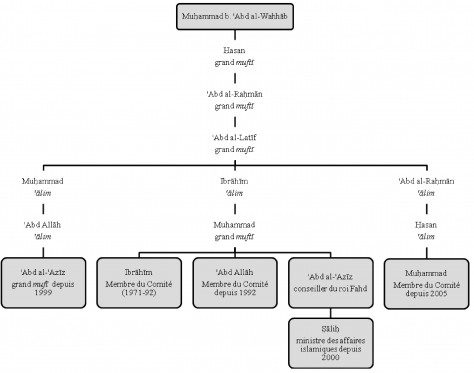
\includegraphics[width=\textwidth]{CourantsIslamContemporain/ImagesCourantsIslamContemporain/genealogie.jpeg}

13 Reste à signaler le cas particulier des oulémas originaires du Hijâz
et d'al-Aḥsā', provinces connues pour leur organisation hétéroclite. En
effet, la plupart des membres du Comité des grands oulémas, originaires
de ces régions, sont issus de ce qu'on a appelé des «dynasties»
d'oulémas, \emph{buyūtāt `ilm}, ou maisons de savoir comme ils aiment
eux-mêmes se faire appeler (à l'instar des familles d'oulémas dans les
autres pays arabes). Plus important encore est le fait que les familles
de ces oulémas appartiennent aux quatre écoles juridiques du sunnisme.
Si le facteur familial revêt une importance certaine, le paramètre de
l'origine tribale doit aussi être pris en compte.
\end{quote}

\hypertarget{la-pruxe9dominance-du-croissant-najdux12b}{%
\section{\texorpdfstring{La prédominance du croissant
\emph{najdī}}{La prédominance du croissant najdī}}\label{la-pruxe9dominance-du-croissant-najdux12b}}

\begin{quote}
14 Force est de constater que l'appartenance à une tribu, généralement
réinventée, constitue un critère identitaire important, dans une société
qui commence à peine à s'individualiser: avant d'être citoyen ou sujet,
on appartient d'abord à une tribu. C'est dire l'importance du milieu
tribal en tant que champ de socialisation des individus. La
\emph{`aṣabiyya}, l'esprit de corps tribal, joue un rôle fondamental
dans le statut social et la promotion de l'individu en Arabie Saoudite.

15 Les oulémas d'origine tribale dominent largement le Comité des grands
oulémas (il s'agit des tribus sédentarisées à partir du e siècle). Ils
sont quarante et un sur les cinquante-deux membres qu'a comptés le
Comité, depuis sa création, à être d'origine tribale, soit 79\%. Les
oulémas d'origine tribale se taillent ainsi la part du lion depuis 1971.
Les onze sièges restants sont occupés par des oulémas issus de trois
milieux différents: des membres de la notabilité citadine du Hijâz
(cooptés pour représenter les intérêts de leur région: on essaie de
choisir les plus «wahhabisés» et/ou quiétistes des oulémas du Hijâz),
des étrangers naturalisés (ils sont hanbalo-wahhabites, ont des talents
«exceptionnels» et ont défendu le hanbalo-wahhabisme et l'État) et des
citadins du Najd, sans affiliation tribale ou \emph{ḫaḍīrī}-s (ces
derniers ne doivent, en principe, leur ascension sociale qu'à leurs
compétences personnelles).

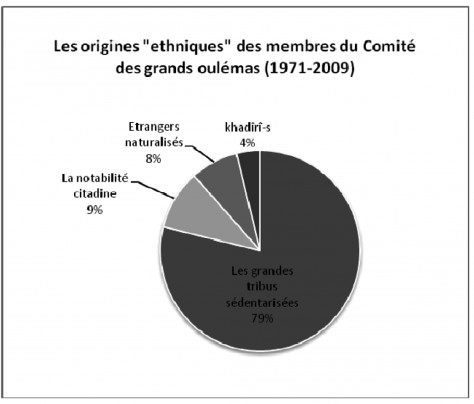
\includegraphics[width=4.9375in,height=4.20833in]{Image/media/image10.jpeg}

16 On constate alors, chiffres à l'appui, que l'appartenance au milieu
tribal sédentarisé joue un rôle déterminant dans l'ascension sociale des
oulémas, la \emph{`aṣabiyya} étant une valeur ajoutée qui permet de se
constituer un capital social. Cela dit, bien que les tribaux dominent
largement en nombre le Comité des grands oulémas, ils ne sont

toutefois pas représentatifs du paysage tribal saoudien. En effet,
certaines tribus comme les Banū Tamīm, les Banū Zayd et les Banū Ḫālid
sont «surreprésentées», tandis que d'autres comme les `Utayba n'ont
guère droit, malgré leur importance numérique, qu'à un seul représentant
au Comité des grands oulémas. D'autres tribus enfin, comme les Šammar,
les Ḥarb, les Muṭayr, les `Ajmān, les Ġāmid, etc. n'ont aucun
représentant au sein du Comité. Si la marginalisation des Šammar, des
`Utayba et des Muṭayr peut s'expliquer par leur passé de tribus
frondeuses, la marginalisation des autres tribus ne peut, elle, être due
qu'à des facteurs religieux et surtout régionaux. Nous nuancerons
seulement, pour finir, en précisant que, dans certains cas, le charisme
personnel du \emph{`ālim} -- c'est le cas d'Ibn Bāz -- fait «oublier»
son appartenance tribale. En effet, ce \emph{`ālim}, citadin sans
affiliation tribale, a pu grimper jusqu'au sommet de l'establishment
hanbalo-wahhabite (il devient grand mufti et président du Comité des
grands oulémas en 1993), uniquement grâce à son «érudition», à son
intégrité morale et à son dévouement aux Sa‛ūd. Le charisme et le
pouvoir symbolique d'Ibn Bāz ont fait de lui le plus grand \emph{`ālim}
hanbalo-wahhabite contemporain.

17 Le royaume d'Arabie Saoudite est un royaume \emph{najdī}. Les élites
saoudiennes sont majoritairement originaires de la région de Najd, fief
de la dynastie et de la doctrine hanbalo-wahhabite. Des études plus
récentes (datant de la dernière décennie) se fondent sur des données
chiffrées mais ne portent que sur les élites ministérielles, la haute
fonction publique et les membres du Conseil consultatif. Rien donc sur
les oulémas. Nous tenterons, dans ce qui suit, de combler ce manque. Sur
les cinquante- deux membres du Comité depuis sa création en 1971, 73\%
des oulémas sont originaires du Najd; 9\% du Ḥijāz, 6\% du Sud, 4\% de
la région orientale et 7\% d'origine étrangère.

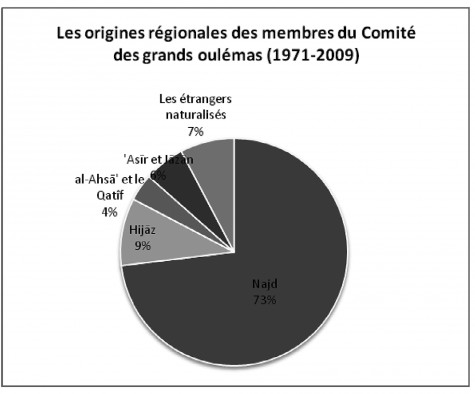
\includegraphics[width=4.94996in,height=4.10417in]{Image/media/image11.jpeg}

18 Une majorité des membres du Comité des grands oulémas est donc
\emph{najdī} et ce depuis sa création. Deux remarques pourraient être
faites à ce propos. La première est que si l'on peut aisément comprendre
que seuls 4\% des grands oulémas sont des Aḥsā'ī-s puisque une grande
partie de la population de cette province est chiite ou sunnite autres
que hanbalo-wahhabite; si l'on peut aussi comprendre que seuls 9\% des
grands oulémas sont \emph{ḥijāzī} puisque, bien que sunnites, ils ne
sont, généralement, pas hanbalo- wahhabites, le chiffre de 6\% seulement
d'oulémas originaires du Sud de l'Arabie Saoudite peut, du moins \emph{a
priori}, paraître absurde puisque les habitants de cette région sont en
majorité hanbalo-wahhabites. L'hypothèse de la préférence régionale peut
être ainsi raisonnablement soutenue: si 73\% des grands oulémas sont
\emph{najdī}, c'est, justement, parce qu'ils sont originaires du fief du
hanbalo-wahhabisme et de la maison
des Sa‛ūd et que, de ce fait, leur soumission à l'un et à l'autre ne
peut être remise en cause. La seconde remarque est que si l'on compare
les chiffres avancés pour le Comité des grands oulémas à ceux que
présente le conseil des ministres au sein duquel les Najdī constituent
72\% des membres (Ibn Ṣunaytān, 2004: 70-73); à ceux du Conseil
consultatif où les Najdī sont majoritaires à 51\% (\emph{ibid}.: 93-96);
à ceux des ministres plénipotentiaires qui sont à 78\% originaires du
Najd ou encore, à ceux des hauts fonctionnaires qui comptent 67\% de
Najdī (\emph{ibid}.: 177-178), on voit que l'élite saoudienne étatique,
qu'elle soit religieuse ou politique, est majoritairement \emph{najdī}.
Les gens du Sud, eux, qui, comme on l'a dit, sont majoritairement
hanbalo-wahhabites, ne représentent que 1\% des ministres, 7\% des
membres de Conseil consultatif, moins de 5\% des ministres
plénipotentiaires et moins de 9\% des hauts fonctionnaires
(\emph{ibid}.: 177- 178): le même raisonnement peut être, ici,
développé. Le régionalisme primerait en Arabie Saoudite. Même si l'on
parle de saoudisation et de formalisation, l'État continue toujours de
s'appuyer sur l'élément najdo-wahhabite pour fonctionner.

19 Observons les chiffres de plus près: lorsque 9\% seulement des
oulémas sont originaires du Hijâz, 20\% des membres du conseil des
ministres, 29\% des membres du Conseil consultatif, 22\% des hauts
fonctionnaires sont \emph{ḥijāzī} (et 34\% parmi eux des cadres
supérieurs). Par ailleurs, en observant les chiffres de plus près
encore, il apparaît qu'au moment de la création du Comité, 29\% des
oulémas sont originaires du Hijâz contre 9\%, nous l'avons dit,
aujourd'hui. Le Comité tend donc, au fur et à mesure qu'il se met en
place et qu'il n'a plus besoin de cadres supérieurs, à se fermer à tout
ce qui n'est pas \emph{najdī}. Il faut ajouter à cela que les oulémas,
quand ils ne sont pas hanbalo- wahhabites, dissimulent leurs croyances
-- ou du moins évitent d'en parler -- et ne jouent, une fois admis au
sein du Comité, qu'un rôle de «figurants».

20 Le Comité des grands oulémas voudrait donner une illusion
d'ouverture: les principales régions sont toutes, même à une faible
proportion, «représentées». Actuellement, deux oulémas d'origine
\emph{ḥijāzi}, deux oulémas originaires du Sud et un autre de l'Est sont
membres du Comité des grands oulémas. En réalité, l'élément \emph{najdī}
domine toujours le Comité, et de loin; de plus, en supposant qu'il y ait
ouverture et même si le Comité accepte en son sein des chiites, il lui
suffirait de conserver une majorité de 51\% de hanbalo-wahhabites
(Najdī) pour que le vote à la majorité absolue passe au sein du Comité
et qu'ainsi, la vision hanbalo-wahhabite continue à dominer.

21 Enfin, en ce qui concerne les oulémas d'origine étrangère, ils ne
sont admis au sein du Comité (au nombre de trois) qu'au moment de la
création de ce Comité. Ces oulémas étrangers étaient, en effet, plus
compétents et plus qualifiés que les oulémas locaux; ils étaient dévoués
à l'État et au hanbalo-wahhabisme; nés non-wahhabites, ils l'étaient
devenus par conviction; ils n'avaient pas d'assise sociale et tribale en
Arabie Saoudite et devaient leur ascension à l'État; enfin, la
solidarité islamique, initiée par le roi Fayçal, entrait également en
ligne de compte. Depuis, le Comité s'est fermé aux étrangers et même les
enfants des dits oulémas étrangers ne sont pas admis au sein du Comité.

22 Le tracé reliant les villes du Najd dont les grands oulémas sont
originaires forme,
pour ainsi dire, un croissant que nous conviendrons d'appeler «croissant
\emph{najdī}» et qui constitue l'épicentre de l'Arabie Saoudite en même
temps que celui du hanbalo- wahhabisme. Il ne faut toutefois pas croire
que si les oulémas du Najd sont largement majoritaires au sein du
Comité, toutes les villes et les régions du Najd y seront équitablement
«représentées». Le Najd compte trois principales régions: la région de
Riyad qui a donné vingt-sept oulémas, le Qaṣīm dix et le Ḥā'il qui n'a
donné aucun \emph{`ālim}. Les deux régions, de Riyad et du Qaṣīm,
offrent un quasi-équilibre dans la répartition des oulémas: dans la
région de Riyad, en dehors de la ville elle-même, qui donne, à elle
seule, sept oulémas, les autres villes donnent, chacune, entre un et
quatre oulémas. De même, dans la région du Qaṣīm, le nombre d'oulémas
par ville varie entre un et trois.

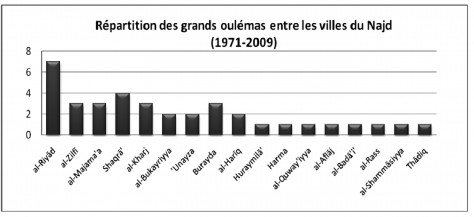
\includegraphics[width=4.9375in,height=2.26042in]{Image/media/image12.jpeg}

23 Le Ḥā'il, quant à lui, est volontairement marginalisé pour une raison
historique évidente: l'émirat du Ḥā'il a longtemps été le rival direct
des Saoud. Nous retrouvons à peine un représentant de cette région dans
le conseil des ministres et un seul autre au Conseil consultatif (Ibn
Ṣunaytān, 2004: 71 et 94).

24 Notons, pour finir, que certaines régions du Najd sont totalement
exclues et n'ont donné aucun \emph{`ālim}: l'exemple d'al-Dawādimī, pour
ne citer que lui, explique ce phénomène dans la mesure où la plupart des
habitants de la ville sont issus de la tribu des `Utayba dont la
fidélité au régime est douteuse. Il y aurait ainsi sous-régionalisation
à l'intérieur même de la régionalisation. De même, aucun grand
\emph{`ālim} n'est issu des régions du Nord. Enfin, aucun chiite n'est
admis au Comité des grands oulémas et ce, pour des raisons évidentes
qu'il ne semble pas utile de rappeler ici. Cela dit, les acquis familial
et tribal, seuls, ne suffisent pas: l'apprenti grand \emph{`ālim} doit
encore suivre un cursus d'études particulier pour intégrer le Comité.
\end{quote}

\hypertarget{de-la-ijux101za-au-doctorat-institutionnalisation-de-la-formation-du-ux101lim}{%
\section{\texorpdfstring{De la \emph{ijāza} au doctorat,
institutionnalisation de la formation du
‛ālim}{De la ijāza au doctorat, institutionnalisation de la formation du ‛ālim}}\label{de-la-ijux101za-au-doctorat-institutionnalisation-de-la-formation-du-ux101lim}}

\begin{quote}
25 Sur les cinquante-deux oulémas qui ont été membres du Comité des
grands oulémas depuis sa création, en 1971, 22\% (soit treize oulémas)
ont reçu une formation traditionnelle et 78\% (soit trente-neuf oulémas)
une formation «moderne». Près d'un quart des oulémas sont ainsi passés
par un cursus traditionnel. Nos entretiens nous permettent de décrire ce
\emph{ta‛līm} et d'en ressortir avec le cursus traditionnel «idéal
typique» du \emph{`ālim} hanbalo-wahhabite.

26 Au départ, entre l'âge de cinq et sept ans, l'apprenti \emph{`ālim}
fait son apprentissage du Coran. Les apprentis oulémas issus d'un milieu
modeste, ceux qui seront plus tard des self-made-men, apprennent le
Coran dans une école coranique (\emph{al-kuttāb}), aux mains d'un cheikh
de renommée moyenne. Les enfants des «cadres religieux moyens» et les
rejetons des dynasties d'oulémas, eux, apprennent le Coran auprès de
leur père, de l'un des membres de leur famille, ou d'un précepteur. On
imagine bien les difficultés rencontrées par les apprentis grands
oulémas issus de milieux modestes et le décalage qui se marque, dès le
départ, entre les apprentis oulémas issus des différentes classes
sociales.

27 Après cette phase d'apprentissage du Coran, l'apprenti \emph{`ālim}
doit, d'une part, commencer à étudier la grammaire et la rhétorique
arabes, de l'autre, apprendre par cœur les trois principaux ouvrages
d'Ibn `Abd al-Wahhāb sur l'unicité divine (\emph{al- tawḥīd}),
fondements du hanbalo-wahhabisme.

28 La troisième étape du cursus classique de l'apprenti \emph{`ālim} est
la quête du savoir
auprès des oulémas réputés. Le futur grand `ālim doit, en effet, réunir
un grand nombre de \emph{ijāzāt} (pl. de \emph{ijāza}: licences), dans
toutes les branches du savoir islamique disponibles, notamment en droit
et en théologie. Il assiste, pour ce faire, plus ou moins
assidûment, à des \emph{ḥalaqāt} `\emph{ilmiyya} ou cercles de savoir,
organisés quotidiennement dans les mosquées ou aux domiciles des
oulémas. Il s'agit alors, de séances de lectures mécaniques suivies de
commentaires d'ouvrages de hadith, d'exégèse coranique, de droit et de
théologie, notamment l'étude des œuvres classiques hanbalites. C'est à
l'issue de ces \emph{ḥalaqāt}, et une fois que l'étudiant a bien retenu
l'ensemble de l'enseignement dispensé par le \emph{`ālim}, qu'il fait un
\emph{istid`ā'}: une demande d'\emph{ijāza} pour les ouvrages étudiés.
Les étudiants les plus brillants deviennent assistants du maître et cela
leur ouvre la porte pour devenir professeur ou juge: la carrière est
alors lancée. Cela a été le cas de Muḥammad al-Sbayyil, le dernier grand
\emph{`ālim} à avoir reçu une formation traditionnelle.

29 Né dans la région du Qaṣīm vers 1926, al-Sbayyil est issu d'une
famille de «cadres religieux moyens». Son père, libraire et copiste
d'ouvrages religieux, connaît parfaitement le Coran. Son frère aîné,
`Abd al-`Azīz, est un \emph{`ālim} de la ville d'al- Bukayriyya. À l'âge
de cinq ans, al-Sbayyil commence son apprentissage du Coran auprès de
son père puis de son frère. Vers l'âge de dix ans, il se lance dans
l'apprentissage des trois ouvrages fondamentaux d'Ibn `Abd al-Wahhāb. Il
étudie aussi la jurisprudence hanbalite sous la direction des oulémas du
Qaṣīm, notamment les ouvrages d'Ibn Taymiyya (m. 1328), d'Ibn Qayyim
al-Jawziyya (m. 1350) et de Mar`ī al- Karamī (m. 1624), etc. À l'âge de
vingt ans, il aurait déjà acquis plusieurs \emph{ijāzāt} qui lui
permirent de devenir l'assistant du juge du Qaṣīm, `Abd Allāh b. Ḥumayd.

30 La formation traditionnelle indispensable au tout début du e siècle
perd, peu à peu, du terrain. En effet, les oulémas qui ont reçu cette
formation s'adaptent difficilement aux exigences de la modernité. 53\%
des membres du Comité des grands oulémas, soit neuf oulémas, ont reçu,
en 1971, une formation dite traditionnelle; en 2009, aucun grand
\emph{`ālim} ne bénéficie d'une telle formation. Dans un pays qui tente
de se moderniser, le besoin d'uniformisation de la formation des grands
oulémas s'impose. Il a fallu, pour y répondre, créer un cursus complet,
homogène, un cursus «national». Nous entendons par cursus moderne, un
cursus «institutionnalisé» et uniformisé.

31 S'ils ne sont que 47\% (soit huit oulémas), en 1971, à suivre la
formation dite moderne,

ils sont aujourd'hui 100\% à le faire. Après un cycle d'études primaires
dans des écoles publiques2\emph{,} les élèves qui se destinent à faire
une carrière juridico-religieuse, rejoignent les instituts de sciences
religieuses (\emph{al-ma`āhid al-`ilmiyya}). Le premier institut voit le
jour à Riyad, en 1950, à l'instigation du grand mufti du royaume de
l'époque, Muḥammad b. Ibrāhīm. Mais très vite, le gouvernement adopte le
projet et les instituts fleurissent dans toutes les régions du royaume
pour atteindre le chiffre de soixante- deux en 2009. Pour accéder à
l'enseignement de ces instituts, l'enfant doit avoir un dossier correct
et avoir appris au moins deux parties du Coran. L'enseignement y est
gratuit. Les instituts de sciences religieuses proposent un cursus de
six années: trois années de collège sanctionnées par un certificat de
réussite, sorte de «brevet» et trois années de lycée sanctionnées par un
certificat de réussite, sorte de «baccalauréat». Les matières étudiées
ont évolué depuis les années cinquante. Au début, l'enseignement était
constitué de quatre troncs communs: les sciences religieuses, les
sciences de la langue arabe, les «sciences sociales», et les
mathématiques. Au fil des années, on a ajouté à ce tronc commun d'études
de base, l'apprentissage obligatoire de la langue anglaise et de
l'informatique. Ces instituts de sciences religieuses sont inégalement
répartis sur l'ensemble du pays: le Najd compte 34\% des instituts, le
Hijâz 13\%, le Sud 28\%, le Nord 18\%, l'Est, enfin, 7\%. Les instituts
sont nombreux dans les régions où le hanbalo-wahhabisme est majoritaire
c'est-à-dire dans le Najd, le Sud et le Nord.

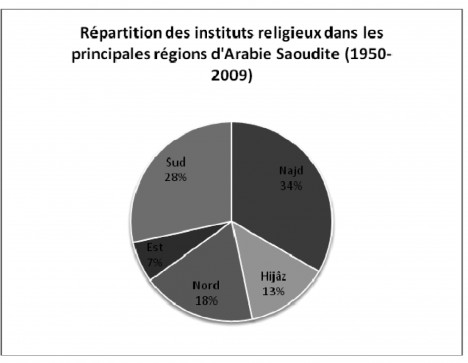
\includegraphics[width=4.875in,height=3.78125in]{Image/media/image13.jpeg}

32 Si la proportion entre le nombre d'instituts créés dans le Hijâz et
celui des oulémas qui sont admis au Comité des grands oulémas est
relativement équilibrée, la proportion entre le nombre d'instituts créés
dans les trois autres régions hanbalo-wahhabites et celui des oulémas
issus de ces régions et effectivement admis au sein du Comité, est,
quant à elle, largement déséquilibrée. On s'attendrait, en effet, à un
nombre plus important d'instituts de sciences religieuses dans le Najd,
à un nombre moins important dans le Sud et à un nombre nul d'instituts
dans la région du Nord. Or, ils sont créés dans le Nord et dans le Sud
mais ce, moins dans le but de former des grands oulémas que dans celui
de «wahhabiser» ces régions en y formant des techniciens du culte
hanbalo-wahhabite et des «cadres religieux moyens».

33 Lorsque l'apprenti \emph{`ālim} a terminé avec succès ses études
secondaires au sein de l'institut, il peut postuler pour les trois
grandes universités du pays: l'Université islamique de Médine (al-Jāmi`a
al-islāmiyya), l'Université islamique de la Mecque (Jāmi`at Umm al-Qurā)
et l'Université islamique de Riyad (Jāmi`at al-imām Muḥammad b. Sa`ūd
al-islāmiyya).

34 La première de ces universités, fondée en 1961, accueille surtout les
musulmans étrangers. Les Saoudiens qui y étudient se destinent
généralement à la prédication à l'étranger. De cette université n'est
issu qu'un seul grand \emph{`ālim}.

35 Quant à la deuxième citée, elle est la plus ancienne université de
théologie d'Arabie Saoudite, fondée en 1949. Elle n'a, malgré son
ancienneté, donnée que six grands oulémas. Doit-on y voir une
manifestation du régionalisme saoudien? Toujours est-il que cette
université accueille, depuis les années soixante-dix, des professeurs,
des cadres et des étudiants de diverses tendances politico-religieuses,
notamment des frères musulmans et des sahwistes (Lacroix, 2010: 47-97)
en lesquels le gouvernement saoudien et le Comité des grands oulémas
n'ont que très peu confiance et qui ne sont donc pas spontanément
recrutés par celui-ci.

36 La dernière université, enfin, est incontestablement la plus
importante pour notre étude. Elle a donné vingt-cinq oulémas, soit 51\%
des membres du Comité, depuis sa création en 1971, et 75\% des oulémas
ayant fait des études universitaires modernes. Cette université naît, en
1974, de la fusion de la faculté de théologie créée, elle, en 1953, et
de la faculté de langue arabe, créée en 1954.

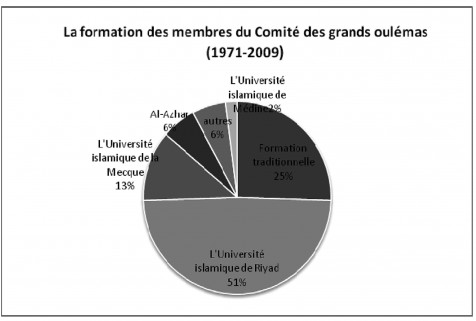
\includegraphics[width=4.95833in,height=3.34375in]{Image/media/image14.jpeg}

37 Depuis sa création, l'Université islamique de Riyad, qui,
rappelons-le, porte le nom du fondateur de l'émirat saoudien Muḥammad b.
Sa`ūd (1744-1765), fidèle allié d'Ibn `Abd al-Wahhāb, est considérée
comme le vivier des grands oulémas et de tous les cadres religieux et
techniciens du culte dont l'establishment religieux a besoin. Le

«pharaonique» campus de l'université (une véritable ville dans la ville
avec ses propres infrastructures, un petit hôpital, un supermarché, des
quartiers résidentiels pour les étudiants, les professeurs et le
personnel administratif, etc.) compte neuf facultés et deux instituts
supérieurs: la faculté de droit {[}musulman{]}; la faculté de théologie;
la faculté de langue arabe; la faculté des sciences sociales
{[}islamiques{]}; la faculté de la prédication et de la communication;
la faculté des langues et de la traduction; la faculté des sciences de
l'informatique; la faculté de l'économie; la faculté des sciences;
l'Institut supérieur de la magistrature et l'Institut de l'apprentissage
de la langue arabe {[}pour les étrangers{]}. Cela dit, les grands
oulémas sont exclusivement issus des facultés de droit et de théologie
et de l'Institut supérieur de la magistrature. Les étudiants dans ces
trois domaines bénéficient d'une bourse d'études et obtiennent, dès la
fin de leur première année d'études, le titre fort apprécié de
\emph{shaykh}. Le succès de l'Université islamique de Riyad est tel que
celle-ci s'est engagée dans une politique d'expansion en développant
deux filiales en Arabie Saoudite3 et cinq à l'étranger4\emph{.} Enfin,
certains étudiants peuvent préparer leur doctorat en sciences
religieuses à l'université égyptienne d'al-Azhar, pour le prestige que
cela donne. Une autre raison pourrait être avancée: certains apprentis
oulémas saoudiens iraient à al-Azhar pour observer l'organisation, les
structures et les mécanismes de fonctionnement de cette prestigieuse
université en vue de les
«importer» en Arabie Saoudite.

38 Les oulémas, au moment de leurs études supérieures, ont tous un tronc
commun tripartite: les fondements de la théologie (\emph{al-`aqīda});
l'exégèse coranique (\emph{al tafsīr}) et la jurisprudence
(\emph{al-fiqh}). À partir de la première année de master (calqué sur le
système anglo-saxon), 74\% des oulémas se spécialisent dans la
jurisprudence, et plus spécialement dans les fondements de la
jurisprudence islamique (\emph{uṣūl al-fiqh}) dans le but d'acquérir la
qualification requise pour émettre des \emph{fatwā}; 26\% d'entre eux,
se spécialisent en théologie, et plus précisément en religions comparées
(en réalité, pour dénigrer toute autre religion que l'islam
hanbalo-wahhabite)5\emph{.} Le choix de ces spécialisations n'est pas
étonnant dans la mesure où les étudiants se destinent avant tout à être
des techniciens du culte et des gestionnaires des biens de salut. Nous
n'entrerons pas, pour ne pas alourdir notre propos, dans le détail des
spécialisations pointues à l'intérieur même des deux grands domaines de
spécialisations que nous avons évoqués.

39 Bien que le cursus moderne se soit bien implanté dans le paysage
saoudien, l'ijāza
n'en demeure pas moins source de prestige et un élément non négligeable
dans un
capital social. Nous avons pu observer que la totalité des oulémas qui
ont suivi le cursus moderne ont, néanmoins, obtenu une ou plusieurs
\emph{ijāzāt}. Elément de prestige comme nous venons de le dire,
l'\emph{ijāza} est, en théorie, facultative. Mais, en pratique,
l'obtention d'une \emph{ijāza} permet au \emph{`ālim}, d'une part, de se
rattacher à une chaîne de transmission
«ininterrompue» d'oulémas remontant jusqu'au Prophète, ce qui permet au
\emph{`ālim} de légitimer sa position et son savoir et de s'inscrire
dans l'héritage prophétique, d'autre part, de nouer des relations
privilégiées avec un ou plusieurs oulémas et de commencer ainsi à tisser
un réseau qui pourra le mener au sommet de l'establishment hanbalo-
wahhabite.

\textbf{Faire carrière: le \emph{cursus honorum} des oulémas}

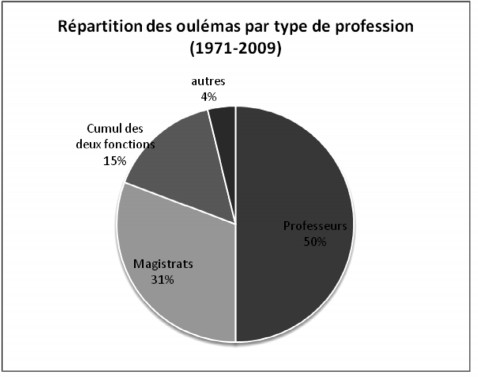
\includegraphics[width=4.97917in,height=3.92708in]{Image/media/image15.jpeg}40
L'enseignement et la magistrature ont toujours été les métiers de
prédilection des oulémas. Les membres du Comité des grands oulémas
n'échappent pas à cette règle. 96\% d'entre eux exercent au moins une de
ces deux professions: 50\% du Comité, soit vingt et un grands oulémas,
ont été ou sont encore, professeurs de jurisprudence islamique ou de
théologie; 31\% d'entre eux sont magistrats dans les différentes
instances de la justice saoudienne; 15\% des grands oulémas ont cumulé
les deux fonctions. À la question: «pourquoi le choix de ces métiers?»
Une première réponse, unanime, des grands oulémas magistrats: «la
justice est le fondement de la royauté». Et, selon les oulémas, qui,
mieux que des spécialistes de «la loi divine», pourraient mettre la
justice en application! Les grands oulémas ont d'ailleurs pleine
conscience de l'importance de leur mission. Ils ont une vision
catastrophiste d'un monde où le \emph{`ilm}, qui risque d'être perdu,
doit être sauvé, épuré des innovations blâmables et transmis par le
\emph{`ālim}.

41 En outre, si la magistrature permet au grand \emph{`ālim} d'observer,
d'analyser et de statuer sur des cas concrets, l'enseignement permet de
transmettre le savoir théorique. Cela, en plus du prestige qui entoure
ces deux fonctions. Il n'est, enfin, pas étonnant de voir que nombre de
grands oulémas cumulent les deux fonctions puisqu'en réalité, l'une et
l'autre sont indissociables (pratique et théorie). Ce phénomène de cumul
des fonctions (d'enseignant et de magistrat) est surtout visible dans la
première génération des grands oulémas. Il s'explique par le manque de
cadres religieux au moment de la
création du Comité. Les grands oulémas devaient donc assumer, tout à la
fois, leur rôle au sein du Comité et les fonctions de magistrats et
d'enseignants. Des années quarante aux années soixante, l'Arabie
Saoudite a été obligée d'«importer» des cadres religieux de l'étranger,
notamment de l'Égypte. Un exemple: l'Égyptien `Abd al-Razzāq `Afīfī (m.
1994), arrivé en Arabie Saoudite, en 1949, pour enseigner la langue
arabe et les sciences religieuses dans un collège à Tayef, a gravi, un à
un, les échelons et parvient au sommet de l'establishment religieux: il
est nommé, en 1971, au sein du Comité des grands oulémas. Cet exemple
révèle deux réalités: premièrement, l'Arabie Saoudite a fait appel aux
étrangers pour l'enseignement, à une certaine époque, à cause du déficit
de cadres dont elle a souffert dans tous les domaines; et deuxièmement,
les étrangers hanbalo-wahhabites, qui pouvaient aisément s'intégrer dans
le pays d'accueil, ont pu, à force de persévérance, atteindre le sommet
de l'establishment religieux saoudien.

42 La pratique du cumul des fonctions d'enseignant et de magistrat tend
à disparaître: le dernier grand \emph{`ālim} à avoir cumulé ces deux
fonctions est `Abd Allāh b. Qa`ūd, membre du Comité de 1977 à
19866\emph{.} Désormais, les grands oulémas, qu'ils soient professeurs
ou magistrats, sont de plus en plus spécialisés, chacun dans son
domaine: de professeurs de droit en général, ils sont devenus
professeurs de droit pénal, de droit de la famille, etc. Parallèlement à
ces deux métiers de prédilection, les grands oulémas sont techniciens du
culte: la plupart d'entre eux sont imâm dans les mosquées. Par exemple,
le grand mufti actuel du royaume, `Abd al-`Azīz āl al-Shaykh, est
également imâm de la grande mosquée de Riyad. Sāliḥ b. Ḥumayd est, lui,
imâm de la grande mosquée de la Mecque, etc. N'oublions pas enfin,
l'autre fonction essentielle des grands oulémas, celle d'«entrepreneurs»
de biens de salut, à savoir promulguer des \emph{fatwā} et se mettre à
l'écoute de la population. Mais si les grands oulémas monopolisent les
grands postes religieux et judiciaires saoudiens, ils n'hésitent pas à
empiéter sur le domaine réservé des autres élites.

43 Une fois admis au sein du Comité, le grand \emph{`ālim} obtient
automatiquement le grade de haut fonctionnaire (\emph{al-martaba
al-mumtāza}), voire celui de ministre. Sur les cinquante-deux membres du
Comité des grands oulémas, vingt-deux ont occupé des postes de
responsabilité autres que ceux de magistrats et d'enseignants. Déjà neuf
membres de la \emph{Hay'a} ont été ou sont encore ministres. Les
ministères que contrôlent les oulémas (si ce ne sont pas eux qui les
contrôlent directement, c'est un membre de l'establishment religieux)
sont ceux de la justice, des affaires islamiques, du pèlerinage et de
l'enseignement des filles (avant le rattachement de ce dernier, en 2002,
au ministère de l'éducation nationale). Depuis sa création, le ministère
de la justice est dirigé par un membre du Comité7\emph{.} Huit membres
du Comité des grands oulémas on été membres du Conseil consultatif: le
président de ce conseil, qui fait se côtoyer islamistes,
«libéraux», conservateurs et tribaux, depuis sa création, en 1992, est
un membre du Comité des grands oulémas. De 1992 à 2002, c'est Muḥammad
b. Jubayr, membre du Comité des grands oulémas (de 1971 à 2002), qui
assure la présidence de cette instance. Sāliḥ b. Ḥumayd, membre du
Comité des grands oulémas depuis 2001, lui succède en 2002. Ce dernier
est remplacé par `Abd Allāh Āl al-Shaykh, en 2009. Trois membres de la
\emph{Hay'a} ont été conseillers du roi Fahd (1982-2005) et deux sont
actuellement conseillers du roi `Abd Allāh. Quatre membres du Comité ont
occupé les postes de doyen ou de président d'université. Par exemple,
`Abd al-`Azīz b. Bāz occupe jusqu'à sa mort, en 1999, le poste de
président de l'Université islamique de Médine. Sa`d al- Ḍuwayḥī est
doyen de la faculté de théologie d'al-Aḥsā'. `Abd Allāh b. `Abd
al-Muḥsin al- Turkī, sans doute l'un des membres les plus actifs du
Comité, actuellement, occupe le poste de président de la Ligue islamique
mondiale, après avoir occupé, entre autres, les postes de président de
l'Université de Riyad et de ministre des affaires islamiques.

44 C'est dire que les oulémas ont adopté, depuis au moins deux
décennies, une stratégie adaptative qui les pousse à investir plusieurs
secteurs d'activités. Outre les domaines religieux, législatif et
éducatif, ils investissent les associations caritatives, les
organisations gouvernementales et non gouvernementales et les domaines
économique et financier. Dans ces deux derniers domaines, trois oulémas,
`Abd Allāh b. Manī`, `Abd
al-Wahhāb Abu Sulaymān et `Abd Allāh al-Muṭlaq se sont «improvisés»
experts et consultants incontournables dans les marchés financiers
saoudiens. Les trois hommes sont aussi membres de plusieurs conseils
d'administration de banques et d'entreprises dans le cadre de ce que
l'on appelle en Arabie Saoudite \emph{al-lijān al-šar`iyya} ou
commissions islamiques. Le nom-même d'un grand \emph{`ālim} sur la
brochure d'une société ou d'une entreprise est la meilleure des
publicités.
\end{quote}

\hypertarget{la-multiplication-des-ruxe9seaux-de-soutien}{%
\section{La multiplication des réseaux de
soutien}\label{la-multiplication-des-ruxe9seaux-de-soutien}}

\begin{quote}
45 Cette mobilité des oulémas n'est, toutefois, possible que si le
\emph{`ālim} tisse, autour de lui, un réseau sur lequel il peut
s'appuyer. Les capitaux culturel et économique doivent encore être
complétés par un réseau de soutiens. Nous avons pu observer trois types
de capitaux sociaux mobilisés par le futur grand \emph{`ālim}. Autrement
dit, le recours aux relations personnelles permet à ce dernier de
s'assurer une meilleure position dans la hiérarchie sociale. Ces trois
réseaux, que nous exposons séparément, sont en réalité, presque
toujours, combinés par le futur grand \emph{`ālim}. Le réseau familial
constitue la première ressource du futur grand \emph{`ālim}. Nous avons,
en effet, constaté l'existence d'au moins trois exemples de réseaux
familiaux qui sont autant de moyens d'accès au Comité des grands
oulémas.

46 Le premier est, sans aucun doute, le plus puissant et le plus dense:
celui des Āl al- Shaykh. Nous avons évoqué plus haut l'importance de
cette famille et nous tenterons, dans ce qui suit, de compléter le
tableau amorcé. L'exemple des deux fils, Ibrāhīm et `Abd Allāh, du grand
mufti Muḥammad b. Ibrāhīm est tout à fait significatif: bien que le
premier des deux ait été relativement peu brillant par rapport aux
collaborateurs de son père, il a quand même été nommé par ce dernier
vice-mufti du royaume d'Arabie Saoudite. Après la mort de son père et la
suppression du poste de mufti, Ibrāhīm, qui était destiné à devenir
mufti, reçoit, en guise de consolation, les postes de ministre de la
justice, de membre du Comité des grands oulémas et de président de la
Direction de la recherche scientifique, de la prédication et de
l'instruction! En 1992, lorsqu'Ibrāhīm se retire des affaires, son
remplaçant au ministère et au Comité des grands oulémas n'est autre que
son frère cadet `Abd Allāh, président actuel du Conseil consultatif. Un
autre exemple étonnant de la famille Āl al-Shaykh: il s'agit de Ṣāliḥ b.
'Abd al-`Azīz, le petit fils d'Ibn Ibrāhīm. Après avoir fait des études
scientifiques depuis le lycée et obtenu un diplôme d'ingénieur, Ṣāliḥ
décide de récupérer l'héritage familial et s'inscrit à l'Université
islamique de Riyad. Grâce à son nom et à l'intervention de son père, qui
était l'un des conseillers du roi Fahd, il obtient une équivalence et
passe ainsi directement en année de master: il contourne la règle qui,
aussi stricte soit-elle, s'efface quand il s'agit d'un Āl al-Shaykh. Il
est actuellement ministre des affaires islamiques et, potentiellement,
membre du Comité des grands oulémas. Un dernier exemple enfin de cette
famille: le dernier admis à Hay'at kibār al-'ulamā', Muḥammad b. Ḥasan,
fait une ascension fulgurante grâce à ses bonnes relations avec son
cousin, le grand mufti actuel d'Arabie Saoudite: il a pu, rapidement,
gravir les échelons universitaires et devenir le directeur de cabinet du
mufti. Ce dernier l'épaule et le soutient: il propose son nom au Comité
des grands oulémas auquel Muḥammad b. Ḥasan accède en avril 2005.
Signalons, enfin, que le réseau familial des Āl al-Shaykh et l'influence
qui en découle, dépassent largement le seul cadre religieux: un membre
de la famille est ambassadeur à Paris, un autre est directeur du
protocole royal, un troisième est membre de la chambre de commerce, etc.
Le deuxième réseau familial est celui des Ibn Ḥumayd, déjà présenté plus
haut.

47 Le dernier réseau familial, enfin, de moindre importance, est celui
des al-Šathrī: cette
famille du Najd a donné quelques oulémas et plusieurs hommes politiques.
`Abd al-‛Azīz al-Šathrī, un des conseillers des rois Fayçal (1964-75) et
Ḫālid (1975-82) a également été un ouléma de renommée moyenne. Son fils,
Nāṣir, a réussi à faire une brillante carrière politique (en tant que
conseiller des rois Ḫālid et Fahd). Selon un des
membres du clan al-Šathrī: «il ne manquait à {[}la{]} famille qu'un
grand \emph{`ālim} pour qu'{[}elle{]} devienne, enfin, une grande
famille». La parentèle met tout en œuvre pour que son rejeton prodige,
Sa‛d, accède au sommet de l'establishment religieux. Aussi, le
prépare-t-on, dès son plus jeune âge, à devenir grand \emph{`ālim} : on
le confie aux maîtres les plus compétents dans le domaine, tels Ibn Bāz,
Ibn `Uthaymīn, al-Aṭram, al-Rakbān et `Abd al-`Azīz Āl al-Shaykh. On le
pousse à s'inscrire à Jāmi'at al-imām où il obtient un doctorat en
fondements de la jurisprudence islamique. Sa`d brûle toutes les étapes
du \emph{cursus honorum} hanbalo-wahhabite et devient professeur de la
même université en un temps records. En mars 2005, la famille soutient
la candidature de son fils au Comité des grands oulémas (le père est
membre du cabinet royal qui transmet les candidatures au roi). Sa`d est
finalement nommé, en avril 2005: à trente-huit ans, il est le plus jeune
membre de l'histoire du Comité des grands oulémas.

48 Nous l'avons dit, le régionalisme et le segmentarisme dominent le
paysage politico- religieux saoudien. La deuxième ressource du futur
grand \emph{`ālim} est, naturellement, le réseau tribal qui va de pair
avec le réseau régional, autrement dit avec le réseau \emph{najdī}. Nous
avons remarqué, en analysant les origines géographiques et tribales des
grands oulémas, que ces derniers sont généralement issus des plus
grandes confédérations tribales du Najd: les Banū Ḫālid ont donné quatre
grands oulémas, les Banū Zayd, sept, les Banū Subay`, trois, les Banū
Tamīm, huit (auxquels il faut ajouter les quatre grands oulémas des Āl
al-Shaykh), les Qaḥṭān, trois, les `Unayza, trois, les Bāhila, deux et
al- Dawāsir, deux également. Soit un total de trente-six grands oulémas
issus des grandes tribus du Najd sur les cinquante-deux membres du
Comité. Le réseau tribal est très dense. Le nombre de grands oulémas est
plus ou moins bien réparti entre les grandes tribus \emph{najdī}. D'un
mouvement de nomination au sein du Comité à l'autre, cet équilibre est,
consciemment ou inconsciemment, maintenu. Exemple: les deux grands
oulémas, Muḥammad āl Sulaymān et Bakr Abū Zayd, de la tribu des Banū
Zayd -- admis tous deux au Comité, en 1992 -- sont remplacés, en 2005,
par deux hommes issus de la même tribu, `Alī al-Ḍuwayḥī et `Abd
al-Raḥmān al-Sadḥān. D'ailleurs, le réseau tribal doublé du réseau
régional ne concerne pas uniquement le champ religieux: on retrouve ces
mêmes configurations dans le domaine politico-administratif (Ibn
Ṣunaytān, 2004, 59-62).

49 La dernière ressource du futur grand \emph{`ālim} est la
\emph{mulāzama}: le fait de s'attacher un
long moment à un maître en sciences religieuses, réputé et influent.
Côtoyer un maître pendant plusieurs années permet à l'apprenti grand
\emph{`ālim} de nouer avec lui des relations personnelles qui peuvent
même aboutir au mariage de l'élève avec la fille ou la nièce du maître.
Par exemple, Ṣāliḥ al-Luḥaydān est, pendant plusieurs années, le
disciple favori du grand mufti Muḥammad b. Ibrāhīm. Cette relation
privilégiée lance véritablement la carrière de Ṣāliḥ qui devient le
gendre et le directeur de cabinet du mufti et qui gagne peu en peu en
charisme. Une année seulement après le décès du maître, al-Luḥaydān est
admis au Comité des grands oulémas; il hérite aussi de la fonction de
magistrat; quelques années plus tard, il devient le président du Haut
conseil de la magistrature, poste qu'il occupe jusqu'en février 2009.
Al-Luḥaydān est le doyen du Comité des grands oulémas dont il est membre
depuis 1971. Il en est aussi un des membres les plus influents. Il
serait, en effet, le seul à pouvoir opposer un veto pour la nomination
d'un nouveau membre: en 2005, il aurait utilisé son veto pour s'opposer
à l'entrée de l'ouléma `Abd al-Muḥsin al-`Ubaykān au Comité.

50 Un autre exemple: Muḥammad al-Sbayyil est le disciple d'Ibn Ḥumayd
alors que
celui-ci est le \emph{qāḍī} d'al-Bukayriyya. Quand Ibn Ḥumayd devient le
\emph{qāḍī} du Qaṣīm, il fait appeler al-Sbayyil à Burayda pour le
désigner professeur et responsable d'un institut de sciences religieuses
de la région. La relation entre les deux hommes est telle que,
lorsqu'Ibn Ḥumayd devient le grand juge du Ḥijāz, il le fait venir à la
Mecque et le nomme imâm de la grande mosquée de la Mecque et
vice-président de l'administration chargée de gérer les deux lieux
saints. Il finit même par en devenir président (jusqu'en 2005) après la
disparition de son protecteur. Depuis son arrivée à la Mecque, il tisse
des
relations étroites avec des oulémas et grands oulémas notamment Ibn Bāz
(qui n'est pas son maître) mais qui finit par lui proposer de devenir
membre du Comité en 1992.

51 Un troisième exemple: c'est également Ibn Bāz qui suit, pas à pas, la
carrière de `Abd
Allāh b. Qa'ūd qui est son meilleur disciple. À la première occasion (le
décès d'Ibn Ḥumayd et de Miḥḍār `Aqīl), Ibn Bāz propose le nom d'Ibn
Qa`ūd au cabinet royal qui le nomme membre du Comité en 1977.

52 Un dernier exemple enfin: le mufti actuel, `Abd al-`Azīz āl
al-Shaykh, en plus du réseau familial que lui confère son nom, bénéficie
du soutien de son maître Ibn Bāz. Il s'agit d'abord d'une question de
solidarité et de reconnaissance: Ibn Bāz est un \emph{mulāzim} du grand
père de `Abd al-`Azīz Āl al-Shaykh, Muḥammad b. `Abd al-Laṭīf. Il aide
donc `Abd al-`Azīz Āl al-Shaykh à devenir professeur à l'université
d'al-Imām, et propose son nom au cabinet royal pour en faire un membre
du Comité des grands oulémas (il le deviendra en 1987). En 1993, Ibn Bāz
devient mufti et désigne `Abd al-`Azīz āl al-Shaykh vice-mufti du
royaume et ce, bien que d'autres grands oulémas soient plus compétents
que lui. En effet, depuis les années soixante et jusqu'à sa mort, en
1999, Ibn Bāz occupe une position-clé dans l'establishment religieux. Il
bénéficie du respect et de la considération des autres grands oulémas et
exerce, de ce fait, une influence autour de lui, tous les grands oulémas
tenant compte de ses conseils et suivant à la lettre ses directives. La
centralité d'Ibn Bāz est ainsi très importante: un grand nombre de
chemins passent par lui. Dix-huit grands oulémas sont ses disciples et
certains d'entre eux lui doivent leur entrée au sein du Comité.
\end{quote}

\hypertarget{le-quiuxe9tisme-politique}{%
\section{Le quiétisme politique}\label{le-quiuxe9tisme-politique}}

\begin{quote}
53 En cherchant à identifier les conditions d'accès au Comité des grands
oulémas à travers le parcours de ses membres, nous avons constaté qu'il
existe deux critères directement liés à la vie politique et sociale:
aucun des grands oulémas n'a de passé politique (c'est-à-dire, une
quelconque manifestation d'opposition au régime: demande de réformes, ou
autres), et aucun \emph{`ālim} n'a jamais critiqué les décisions du
Comité ou de l'un de ses membres et ce, même si ses positions allaient à
l'encontre des décisions officielles.

54 `Abd Allāh Ibn Jibrīn, haut fonctionnaire religieux et candidat
potentiel au Comité des grands oulémas, a été l'un des parrains de la
contestation islamiste des débuts des années quatre-vingt-dix (Kepel,
2003: 335-337; Lacroix, 2007: 371-443). Ces actes constituent une
véritable offense tant pour le régime que pour les grands oulémas. Ces
derniers ne manquent pas, d'ailleurs, de le désavouer publiquement: il
est démis de ses fonctions officielles. Réhabilité par la suite, et bien
que très bon \emph{`ālim}, il ne pourra cependant jamais prétendre au
poste de grand \emph{`ālim} en raison de cette «bavure»: s'étant
ouvertement opposé au gouvernement et ayant participé à des activités
politiques allant à l'encontre des positions officielles, son «rachat»
et son récent soutien au gouvernement ne suffisent pas. Il ressort de
cet exemple que le quiétisme politique des candidats au Comité est un
élément fondamental et un critère-clé de sélection. Tout ce que peut
tolérer le Comité comme engagement politique pour un futur grand
\emph{`ālim} est le soutien aux décisions du pouvoir. `Alī al-Ḍuwayḥī
est l'exemple du \emph{`ālim} engagé politiquement -- en faveur du
régime bien sûr -- qui accède à la Hay'a. En effet, depuis 2001,
al-Ḍuwayḥī, qui dirige la faculté de théologie d'al-Aḥsā', a signé
plusieurs pétitions politiques défendant les programmes scolaires
saoudiens, et se déclarant en faveur de la tenue d'élections
municipales, etc.

55 Quant à `Abd al-Muḥsin al-`Ubaykān, qui a appelé ouvertement le
gouvernement à entreprendre des réformes, entre 1992 et 1994, il a été
marginalisé et démis de ses multiples fonctions: il perd son poste de
juge au tribunal de Riyad et d'imâm de mosquée. Réhabilité, dans les
années 1999-2000, il continue néanmoins à critiquer les décisions de la
Hay'a (surtout celles qui concernent la jurisprudence), et du système
judiciaire. Il émet même des \emph{fatwā} contredisant celles du Comité
des grands oulémas et
tente, pour se rattraper, de promulguer des \emph{fatwā} sur la licéité
du salut du drapeau national, sur la condamnation des sahwistes ou
encore sur l'interdiction du djihâd en Irak pour les Saoudiens. Le
gouvernement a accepté de le réhabiliter mais les oulémas ont opposé un
veto catégorique à l'entrée de ce \emph{`ālim} au Comité. Al-`Ubaykān a,
finalement, été nommé, dans un premier temps, conseiller au ministère de
la justice et membre du Conseil consultatif, avant de devenir l'un des
conseillers du roi, en 2009.

56 Les leaders de la \emph{ṣaḥwa} dans les années quatre-vingt-dix,
Safar al-Ḥawālī, Salmān al-`Awda et Muḥsin al-`Awājī, reconnaissent
eux-mêmes que l'un des critères d'accès au Comité des grands oulémas est
le quiétisme sur les plans politique et sécuritaire et acceptent donc,
du fait de leur très grand engagement politique, de ne pas y prétendre.

«Pour le gouvernement, dit al-Ḥawālī, les grands oulémas doivent être
des hommes apolitiques, des hommes qui ignorent tout de la politique».
Salmān al-`Awda ajoute que

«les futurs membres du Comité doivent être des hommes sans histoire(s)».
Pour Muḥsin al-`Awājī «l'accès au Comité obéit à des critères purement
sécuritaires».

57 Il découle de tout cela le «portrait idéal» du membre du Comité des
grands oulémas:

le grand \emph{`ālim} est hanbalo-wahhabite; il est issu d'une famille
de «cadres religieux moyens» ou d'une «dynastie» d'oulémas; il est issu
d'une grande tribu sédentarisée du croissant \emph{najdī}; il a effectué
des études auprès de maîtres réputés (cela pour le \emph{`ālim} qui suit
une formation traditionnelle) ou dans un \emph{ma`had `ilmī} puis à
l'université al-Imām de Riyad (pour le grand \emph{`ālim} qui a reçu une
formation moderne); il s'est spécialisé en jurisprudence islamique; il
est généralement professeur d'université (al-Imām) ou magistrat; il a en
moyenne vingt-cinq années d'expérience dans le domaine religieux; il
n'est pas engagé politiquement (s'il l'est, il ne doit l'être qu'en
faveur du régime).

58 La moyenne d'âge du grand \emph{`ālim} qui accède au Comité est de
quarante-sept ans. Il y reste en moyenne quinze ans. Et, si les
circonstances d'accès à la Hay'a sont difficiles à déterminer, les
circonstances de départ de la Hay'a sont, elles, tout à fait claires: le
grand \emph{`ālim} quitte le Comité s'il décède, bien évidemment, s'il
est gravement malade ou s'il a commis un acte jugé répréhensible par le
roi -- en 1992, quatre grands oulémas auraient refusé de signer une
\emph{fatwā} et ont été limogés.

59 Le renouvellement des membres du Comité des grands oulémas est
généralement associé à une période de crise ou de transition. Les
renouvellements de 1987 et de 2001 sont des renouvellements de
transition (plusieurs oulémas sont décédés ou gravement malades), les
renouvellements de 1992 et 2005 coïncident avec des moments de crise
(respectivement, les conséquences de la guerre du Golfe et celles du 11
septembre). Depuis la création de la Hay'a, il y a eu reproduction de
l'élite: il ne reste plus de la génération de 1971 que trois membres.
Nous constatons toutefois que l'élite des grands oulémas restreint
l'accès, même à des personnes qui rempliraient toutes les conditions
formelles pour accéder au Comité. Sans doute le prestige d'appartenir au
Comité des grands oulémas ne pourrait que diminuer si l'accès devenait
trop aisé. L'élite du Comité est donc fermée: cinquante-deux membres en
trente-huit ans.
\end{quote}

\hypertarget{conclusion}{%
\section{Conclusion}\label{conclusion}}

\begin{quote}
60 L'habitus, ainsi défini, des grands oulémas, fruit d'un
conditionnement historique et social, est générateur d'un comportement
adapté, consciemment ou inconsciemment, à la logique de l'espace
politico-religieux saoudien: soutenir le pouvoir politique et gérer le
marché officiel des biens de salut. Les larges prérogatives dont dispose
le Comité dans les domaines politique, social et religieux, à côté de sa
fonction fondamentale de bastion idéologique et d'usine à légitimer les
actions du gouvernement, justifient le contrôle par le pouvoir politique
de son ordre du jour et de son budget et conditionnent le choix, très
sélectif, de ses membres. Les grands oulémas, qui se définissent eux-
mêmes comme les oulémas du pouvoir, doivent être acquis au régime. Si
les origines sociales, le parcours éducatif et les réseaux de
socialisation favorisent l'émergence d'une élite fermée et dévouée au
pouvoir, la `\emph{aṣabiyya} régionale y est pour beaucoup. Le

Comité est, à l'instar des autres institutions du pays, trusté par
l'élément \emph{najdī} (plus de 70\% des membres des élites saoudiennes
sont \emph{najdī}): cette région n'est-elle pas le fief du
hanbalo-wahhabisme et de la dynastie régnante? Il s'agit enfin pour les
oulémas d'un dévouement objectif: les intérêts spirituels et temporels
de l'establishment religieux étant intrinsèquement liés à ceux du
régime, si ce dernier était mis à mal, la domination du
hanbalo-wahhabisme sur le territoire saoudien -- très éclectique
religieusement -- serait indubitablement remise en cause.
\end{quote}

